\subsection{Einführung}
Für das gestalten der grafischen Oberfläche wurde bei \sblit \acrshort{swt} verwendet.
Das Standard Widget Toolkit ist eine Open-Source-Bibliothek für grafische
Benutzeroberflächen entwickelt von Eclipse. Es unterstützt viele Plattformen,
darunter Windows 2000/XP/Vista/7/8, Linux und Mac OS X und bietet eine
Programmschnittstelle, die es eralubt, auf die nativen Widgets des
Betriebssystems zuzugreifen, sofern dies möglich ist. Zusätzlich werden noch
weitere Widgets angeboten, die nicht nativ existieren, aber in dem
Betriebssystem-spezifischen Design gehalten sind, wie zum Beispiel das Tree-
oder Table-Widget.

\subsection{Vorteile}
\begin{description}
	\item[{Behält Design der jeweiligen Plattform}]
    Damit eine möglichst große Reichweite mit \sblit erreicht werden kann, wurde bei
    besonders auf Plattformunabhängigkeit geachtet, um \sblit mit wenig
    Anpassungsaufwand auf verschiedensten Betriebssystemen laufen lassen zu können.
		\acrshort{swt} hat nun den Vorteil, dass es auf den verschiedenen Plattformen das
    spezifische Aussehen des jeweiligen Betriebssystems hat, obwohl das selbe
    Programm ausgeführt und die selben Elemente verwendet werden.

	\item[{Einsteigerfreundlicher Editor}]
    Sich mit einem neuen Framework zu beschäftigen kostet Zeit und Energie. Um
    diesen Schritt zu erleichtern, gibt es für die meisten Frameworks für grafische
    Oberflächen einen \gls{wysiwygeditor}. So auch bei \acrshort{swt}, weshalb
    sich die Einarbeitungsphase einfacher gestaltet, als dies bei manch anderen Frameworks
    der Fall ist.
\end{description}

\subsection{Nachteile}
\begin{description}
	\item[{Ist auf Linux weniger performant}]
    Auf allen Plattformen außer Windows (wie zum Beispiel Linux) ist \acrshort{swt} manchmal
    weniger performant, da bestimmte Widgets nicht vorhanden sind und erst emuliert werden müssen.

	\item[{Ist nicht \acrshort{mvc} basiert}]
    SWT basiert nicht auf einem \acrshort{mvc}-Design, bietet mit JFace allerdings eine
    \acrshort{mvc}-Abstraktion als Erweiterung.
\end{description}

\subsection{Aufbau}
Der Aufbau bei \acrshort{swt} ist sehr einheitlich. Es gibt zwei Hauptelemente:
\code{Display} und \code{Shell}. Jedes Element hat ein Partnerelement als Parameter
und jedes Widget noch dazu ein Stil-Bit, dass dem Element eine vordefinierte Optik
verleiht. Zudem gibt es noch Container-Klassen, auf die ein Layout angewendet werden
kann, um die ihm untergeordneten Elemente zu positionieren.
\listingstart{Beispielklasse für grafische Oberfläche \datei{erklaerungsGUI}}
public class erklaerungsGUI {
	Display display;
	Shell shell;

	public static void main(String[] args) {
		new erklaerungsGUI();
	}

	public erklaerungsGUI(){
		display = new Display();
		shell = new Shell(display);

		GridLayout layout = new GridLayout(2, false);
		shell.setLayout(layout);

		Button pushButton = new Button(shell, SWT.PUSH);
		GridData layoutData = new GridData(SWT.FILL, SWT.FILL, true, true, 1, 1);
		pushButton.setLayoutData(layoutData);
		pushButton.setText("Push");

		Button arrowButton = new Button(shell, SWT.ARROW);
		layoutData = new GridData(SWT.FILL, SWT.FILL, true, true, 1, 1);
		arrowButton.setLayoutData(layoutData);

		shell.setSize(200, 100);
		shell.open();

    // Eventloop
		while (!shell.isDisposed()) {
			if (!display.readAndDispatch())
				display.sleep();
		}
		display.dispose();
	}
}
\end{lstlisting}

\begin{description}
	\item[{Display}]
    Die \code{Display}-Klasse ist einer der Kernkomponenten innerhalb einer \acrshort{swt}-\acrshort{GUI}.
    Sie verwaltet Event-Loops, Schriftarten, Farben und die generelle Kommunikation zwischen dem \acrshort{GUI}-Thread
    und den anderen Threads. Jedes Programm mit einer \acrshort{swt}-\acrshort{GUI} muss ein \code{Display}-Objekt haben.

    \item[{Shell}]
    Die \code{Shell}-Klasse ist die zweite der Kernkomponenten einer \acrshort{swt}-\acrshort{GUI}.
    Sie stellt das Programmfenster dar und wird das Elternelement aller eingefügten Widgets.
		Das \code{Display}-Objekt muss ein oder mehrere \code{Shell}-Objekte als Unterobjekt haben.
    Mit der Funktion \code{shell.open()} wird das Programmfenster erst gezeichnet.

    \item[{GridLayout}]
    Layouts können auf \code{Composite}-Objekte angewandt werden, um die darin befindlichen
		Elemente zu positionieren. Ein Beispiel für ein Solches Objekt ist die \code{Shell}.
    Es gibt verschiedenste Layouttypen, je nach Struktur, in der man die Elemente anordnen will.
    Um jedem Widget eine Layoutinformation, also unter anderem eine Position zuordnen zu können,
		die jeweilig spezielle \code{LayoutData} benötigt.

    \item[{Button}]
    Zwei typische Buttons als Beispiel-Widgets. Als Parameter wird die Shell als
    Elternelement angegeben und \code{SWT.PUSH} beziehungsweise \code{SWT.ARROW}
    als Stil-Bit. Dieser unterschiedliche Parameter erklärt auch die andere Optik
    der Buttons.

    \item[{Eventloop}]
    Damit das \acrshort{GUI} nicht sofort geschlossen wird, gibt es diese Eventloop.
		Eine Schleife, die wartet bis ein gewisses Event eintritt. In diesem Fall wird
		darauf gewartet, dass das Fenster, also das \code{Shell}-Objekt disposed, also
		geschlossen wird.

\end{description}

\begin{figure}[htb]
	\centering
	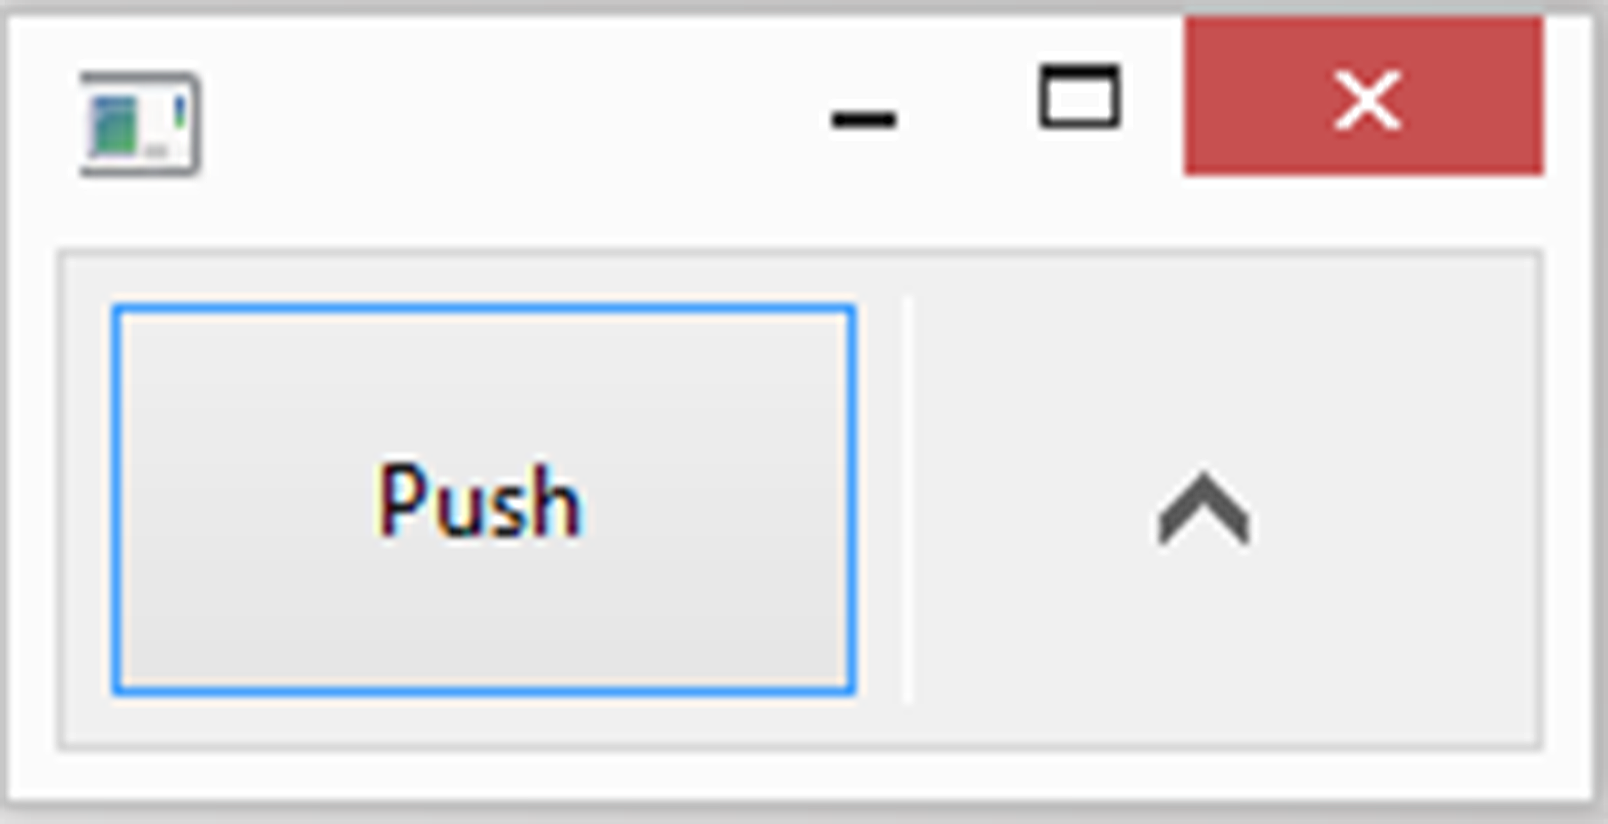
\includegraphics[]{images/erklaerungsgui.png}
	\label{erklaerungsgui}
  \caption{Beispiel-\acrshort{GUI} zur Erklärung}
\end{figure}
